\documentclass[a4paper]{article}
\usepackage[fontsize=13pt]{scrextend}
\usepackage[utf8]{vietnam}
\usepackage{amsmath}
\usepackage{amsfonts}
\usepackage{xcolor}
\usepackage{titlesec}
\usepackage{mdframed}
\usepackage{amssymb}
\usepackage{pgf,tikz,pgfplots}
\usepackage{graphicx}
\graphicspath{ {../figures/} }
\usepackage{array}
\usepackage{cases}
\usepackage{listings}
\usepackage{tabulary}
\usepackage{color}
\usepackage{float} 
\usepackage{hyperref}
\usepackage{multirow}
\usepackage{minitoc}
\pgfplotsset{compat=1.5}
\usepackage{mathrsfs}
\usetikzlibrary{arrows, calc}
\usepackage{fancyhdr}
\pagestyle{fancy}
\pagestyle{empty}
\usepackage[noend]{algpseudocode}
\usepackage{algorithm,algpseudocode}
\usepackage{lipsum}
\makeatletter
\newenvironment{breakablealgorithm}
  {% \begin{breakablealgorithm}
   \begin{center}
     \refstepcounter{algorithm}% New algorithm
     \hrule height.8pt depth0pt \kern2pt% \@fs@pre for \@fs@ruled
     \renewcommand{\caption}[2][\relax]{% Make a new \caption
       {\raggedright\textbf{\fname@algorithm~\thealgorithm} ##2\par}%
       \ifx\relax##1\relax % #1 is \relax
         \addcontentsline{loa}{algorithm}{\protect\numberline{\thealgorithm}##2}%
       \else % #1 is not \relax
         \addcontentsline{loa}{algorithm}{\protect\numberline{\thealgorithm}##1}%
       \fi
       \kern2pt\hrule\kern2pt
     }
  }{% \end{breakablealgorithm}
     \kern2pt\hrule\relax% \@fs@post for \@fs@ruled
   \end{center}
  }
\makeatother
\definecolor{dkgreen}{rgb}{0,0.6,0}
\definecolor{gray}{rgb}{0.5,0.5,0.5}
\definecolor{mauve}{rgb}{0.58,0,0.82}
\usepackage[
    backend=biber,
    style=numeric,
    natbib=true,
    url=true, 
    doi=true,
    eprint=false,
    sorting=nyt
]{biblatex}
\addbibresource{refs.bib}
\lstset{frame=tb,
  language=Python,
  aboveskip=3mm,
  belowskip=3mm,
  showstringspaces=false,
  columns=flexible,
  basicstyle={\small\ttfamily},
  numbers=none,
  numberstyle=\tiny\color{gray},
  keywordstyle=\color{blue},
  commentstyle=\color{dkgreen},
  stringstyle=\color{mauve},
  breaklines=true,
  breakatwhitespace=true,
  tabsize=3
}
\renewcommand{\listfigurename}{Danh sách hình}
\renewcommand{\listtablename}{Danh sách bảng}
\newcommand{\tabitem}{~~\llap{\textbullet}~~}
\usepackage[left=2cm,right=2cm,top=2cm,bottom=2cm]{geometry}
\author{Nguyễn Văn Lộc}
\newmdenv[linecolor=black,skipabove=\topsep,skipbelow=\topsep,
leftmargin=-5pt,rightmargin=-5pt,
innerleftmargin=5pt,innerrightmargin=5pt]{mybox}
\begin{document}
%Order of compilation (on TexMaker): F6 (pdfLaTex) -> F11 (BibTex) -> F6 (pdfLaTex) -> F7 (view pdf)
\fancyhf{}
\lhead{Báo cáo đồ án Toán ứng dụng và thống kê}
\chead{}
\rhead{Mô hình Markov ẩn}
\cfoot{\thepage}
\rfoot{}
\lfoot{}
\pagestyle{fancy}
\begin{titlepage}
\begin{mybox}
\begin{center}
\fontsize{12}{12}\selectfont
\textbf{ĐẠI HỌC QUỐC GIA THÀNH PHỐ HỒ CHÍ MINH}\\
\textbf{TRƯỜNG ĐẠI HỌC KHOA HỌC TỰ NHIÊN}\\
\textbf{KHOA CÔNG NGHỆ THÔNG TIN}
\end{center}
\vskip 0.5 cm
\begin{figure}[H]
\begin{center}

\includegraphics[scale=0.25]{../figures/logo}
\end{center}
\end{figure}
\vskip 0.5 cm
\begin{center}
\fontsize{18}{14}\selectfont
\textbf{BÁO CÁO ĐỒ ÁN MÔN HỌC}\\
\fontsize{24}{16}\selectfont
\textbf{TOÁN ỨNG DỤNG VÀ THỐNG KÊ}\\
\fontsize{18}{12}\selectfont
\textbf{Chủ đề: Mô hình Markov ẩn}
\end{center}
\vskip 1 cm
\fontsize{14}{12}\selectfont
\textbf{Giảng viên lý thuyết:} PGS. TS. Nguyễn Đình Thúc\\
\textbf{Giảng viên hướng dẫn thực hành:}
\begin{itemize}
\item Thầy Nguyễn Văn Quang Huy
\item Cô Võ Nam Thục Đoan
\end{itemize}
\textbf{Lớp:} 20TN\\
\textbf{Thành viên thực hiện:}
\begin{itemize}
\item 20120131 $-$ Nguyễn Văn Lộc
\item 20120536 $-$ Võ Trọng Nghĩa
\item 20120572 $-$ Nguyễn Kiều Minh Tâm
\end{itemize}
\vskip 3 cm
\begin{center}
\textbf{THÀNH PHỐ HỒ CHÍ MINH, THÁNG 4-5 NĂM 2022}
\end{center}
\end{mybox}
\end{titlepage}
\newpage

\section*{Lời nói đầu}
\nocite{hmm2021}
\newpage

\tableofcontents
\newpage

\section{Lý thuyết mô hình Markov ẩn}
Mô hình Markov ẩn (Hidden Markov model $-$ HMM) là một mô hình máy học cổ điển thông dụng trong việc xử lý chuỗi.
\subsection{Các thành phần của một mô hình Markov ẩn là gì? Chúng khác gì với mô hình Markov?}
Một mô hình Markov ẩn có cấu tạo như sau \supercite{angrybird, hmm2021}:
\begin{mybox}
\begin{itemize}
\item $Q = {q_1}{q_2} \ldots {q_N}:$ tập hợp $N$ trạng thái (states).
\item $A = {a_{11}} \ldots {a_{ij}} \ldots {a_{NN}}:$ ma trận xác suất chuyển (transition probability matrix) $A,$ $a_{ij}$ là xác suất chuyển từ trạng thái $i$ sang trạng thái $j,$ $\sum\limits_{j = 1}^N {{a_{ij}}}  = 1,\forall i.$
\item $O = {o_1}{o_2} \ldots {o_T}:$ chuỗi các quan sát (observations), lấy từ bộ từ vựng (vocabulary) $V = {v_1}, {v_2}, \ldots, {v_V}.$
\item $B = b_i \left( {o_t} \right):$ ma trận xác suất phụ thuộc trạng thái (emission probabilities), thể hiện xác suất một quan sát $o_t$ được tạo thành từ trạng thái $i.$
\item $\pi = {\pi_1}, {\pi_2}, \ldots, {\pi_N}:$ phân phối xác suất ban đầu theo trạng thái, có nghĩa là $\pi_i$ thể hiện xác suất xích Markov bắt đầu ở trạng thái $i.$ Một số trạng thái $j$ có thể có $\pi_j = 0,$ do chúng không thể là trạng thái ban đầu của xích Markov.
\end{itemize}
\end{mybox}
So với xích Markov (Markov chains), mô hình Markov ẩn có thêm 2 thành phần là $O$ $-$ chuỗi các quan sát và $B$ $-$ ma trận xác suất phụ thuộc trạng thái.


\subsection{Các giả thiết (assumptions) đặt ra cho mô hình Markov ẩn là gì? Tìm ví dụ các bài toán mà các giả thiết này hợp lý và bất hợp lý.}
\textbf{Các giả thiết (assumptions) đặt ra cho mô hình Markov ẩn.}\\
Một mô hình Markov ẩn có 2 giả thiết chính:
\begin{itemize}
\item Xác suất của một trạng thái cụ thể chỉ phụ thuộc vào trạng thái ngay trước đó (Markov Assumptions):
\begin{equation}
 P\left({\left. {{q_i}} \right|{q_1} \ldots {q_{i - 1}}} \right) = P\left( {\left. {{q_i}} \right|{q_{i - 1}}} \right).
\end{equation}

\item Xác suất của một quan sát \(o_i\) chỉ phụ thuộc vào trạng thái tương ứng sinh ra nó \(q_i\) chứ không phụ thuộc vào bất kỳ trạng thái \(q_j\) nào khác hay bất kỳ quan sát \(o_k\) nào.
\begin{equation}
P\left({\left. {{o_i}} \right|{q_1}, \ldots {q_{i}}\ldots ,q_T,o_1,\ldots,o_i,\ldots,o_T} \right) = P\left( {\left. {{o_i}} \right|{q_i}} \right).
\end{equation}

\end{itemize}

Ví dụ bài toán mà giả thiết cho mô hình Markov ẩn hợp lý:

Ví dụ bài toán mà giả thiết cho mô hình Markov ẩn bất hợp lý:

\subsection{Cho một mô hình Markov ẩn với các tham số đã biết, thuật toán tiến trước (forward algorithm) được dùng để xác định độ hợp lý (likelihood) của một chuỗi quan sát (observation). Mô tả và đánh giá độ phức tạp của thuật toán tiến trước.}

Xét mô hình Markov ẩn \(\lambda = (A,B)\) và chuỗi các quan sát \(O\), hãy xác định độ hợp lý (likelihood) của nó \(P(O|\lambda)\).

Thuật toán tiến trước sử dụng một bảng để lưu trữ các giá trị trung gian và tính toán xác suất xảy ra một quan sát nào đó thông qua việc lấy tổng của tất cả các trường hợp có thể xảy ra của tập các trạng thái "ẩn" có thể đưa đến quan sát tương ứng, thực hiện tính toán trên tập các đường đi tạo thành một "lưới".

Mỗi mắt xích trong "lưới" của thuật toán này, \(\alpha_t(j)\) thể hiện xác suất ở trạng thái \(j\) sau khi trải qua \(t\) quan sát đầu tiên, với mô hình \(\lambda\) đã biết, nói cách khác, \[\alpha_t(j) = P(o_1,o_2,\ldots,o_t,q_t = j|\lambda)\], và giá trị này được tính dựa trên các đường đi dẫn đến mắt xích này và lấy tổng, tức là \[\alpha_t(j) = \displaystyle\sum_{i=1}^{N}\alpha_{t-1}(i)a_{ij}b_j(o_t)\]

Trong đó: \(\alpha_{t-1}(i)\) chính là xác suất trên đoạn đường đến ô này, \(a_{ij}\) là xác suất chuyển tiếp từ trạng thái \(q_i\) sang trạng thái hiện tại \(q_j\), và \(b_j(o_t)\) là độ hợp lý của trạng thái quan sát \(o_t\) ứng với trạng thái hiện tại \(j\).

Sau đây là mô tả thuật toán tiến trước:

\begin{breakablealgorithm}
  \caption{Thuật toán tiến trước}
  \begin{algorithmic}[1]
    \Function{Forward}{$observations \text{ of len } T, stategraph \text{ of len } N$} \Return $forwardprob$

    \State $\text{tạo một ma trân xác suất đường đi } forward[N, T]$
    \State \Comment{khởi tạo}
    \For {$\text{mỗi trạng thái } s$ \textbf{from} $1$ \textbf{to} $N$}
        \State $forward[s,1] \gets \pi_s * b_s \left( {o_1} \right)$
        \State \Comment {đệ quy}
     \EndFor
     \For {$\text{mỗi bước}$ $t$ \textbf{from} $2$ \textbf{to} $T$}
        \For {$\text{mỗi trạng thái } s$ \textbf{from} $1$ \textbf{to} $N$}
        	\State $forward[s, t] \gets \displaystyle\sum_{s' = 1}^N \left( {forward\left[ {s',t - 1} \right]*{a_{s',s}}*{b_s}\left( {{o_t}} \right)} \right)$
        \EndFor
      \EndFor
      \State $forwardprob \gets \displaystyle\sum_{s = 1}^N forward[s,T]$
     \State \Comment{Kết thúc}

    \Return $forwardprob$
    \EndFunction
  \end{algorithmic}
\end{breakablealgorithm}

Trong giải thuật nói trên, giá trị \(forward[s,t]\) chính là giá trị \(\alpha_t(s)\) trình bày ở nội dung trước cùng đề mục. Các bước thực hiện được tóm lại như sau:

1. Khởi tạo: gán các \[\alpha_1(j) = \pi_jb_j(o_1),\forall 1\le j\le N\] (các dòng 4, 5 trên mã giả)

2. Tính toán truy hồi: tính các \[\alpha_t(j) = \displaystyle\sum_{i=1}^{N}\alpha_{t-1}(i)a_{ij}b_j(o_t); \forall 1\le j\le N, 1<t\le T\] (các dòng 7, 8, 9 trên mã giả)

3. Kết thúc: giá trị cần tính \[P(O|\lambda) = \displaystyle\sum_{i=1}^{N}\alpha_{T}(i)\] (chính là giá trị \(forwardprob\) đề cập trong thuật toán)

Giải thuật có độ phức tạp thời gian là \(O(N^2T)\) trong đó \(N,T\) tương ứng là độ dài của tập trạng thái và độ dài của dãy quan sát cần tính toán giá trị độ hợp lý (likelihood) này; và là \(O(NT)\) cho không gian lưu trữ (bảng tạm $forward$).

\subsection{Cho một mô hình Markov ẩn với các tham số đã biết, thuật toán Viterbi được dùng để xác định chuỗi trạng thái (state) khả dĩ nhất. Mô tả và đánh giá độ phức tạp của thuật toán Viterbi.}
Với mỗi mô hình chứa những biến ẩn (hidden variables), chẳng hạn như mô hình Markov ẩn, việc quyết định chuỗi biến nào là nền tảng (underlying source) của một (vài) chuỗi quan sát gọi là \textbf{giải mã} (decode). Công việc này được thực hiện bởi một \textbf{decoder}.\\
\begin{mybox}
\textbf{Giải mã (Decoding):} cho một mô hình Markov ẩn $\lambda = \left( {A, B} \right)$ và một chuỗi các quan sát $O = o_1, o_2, ..., o_T,$ tìm chuỗi các trạng thái $Q = {q_1}{q_2}{q_3}...{q_T}$ có khả năng xảy ra nhất.
\end{mybox}
Ta có thể đưa ra chuỗi tốt nhất như sau: với mỗi chuỗi trạng thái ẩn có thể, ta có thể sử dụng thuật toán tiến trước và tính độ hợp lý của chuỗi quan sát có được từ chuỗi trạng thái ẩn đó. Sau đó, ta có thể chọn chuỗi với độ hợp lý cao nhất. Dễ thấy từ phần trước rằng ta không thể làm theo cách này vì số lượng chuỗi trạng thái có thể là hàm mũ.\\
Thay vào đó, thuật toán giải mã phổ biến nhất là \textbf{thuật toán Viterbi} (Viterbi algorithm). Giống như thuật toán tiến trước, Viterbi là một thuật toán quy hoạch động sử dụng dynamic programming trellis. Viterbi cũng thể hiện một biến thể của quy hoạch động, thuật toán minimum edit distance.
\begin{figure}[H]
\begin{center}
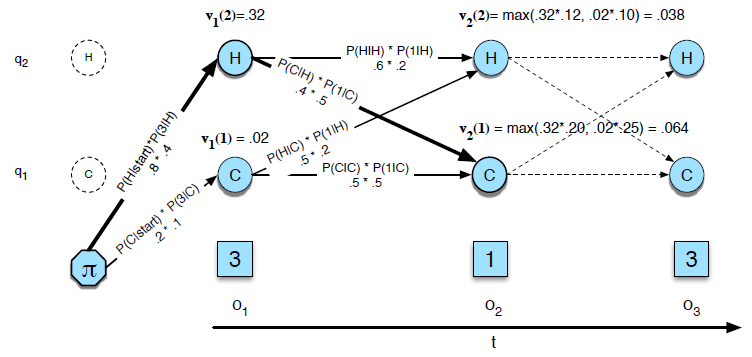
\includegraphics[scale=1]{viterbi/fig1}
\end{center}
\caption{Viterbi trellis dùng cho việc tìm đường đi tốt nhất qua các không gian trạng thái ẩn cho việc ăn kem. Các trạng thái ẩn được đóng khung trong vòng tròn, các quan sát được đóng khung hình vuông. Các hình tròn nét đứt màu trắng thể hiện. Hình trên thể hiện quá trình tính $v_i \left( j \right)$ cho 2 trạng thái ở 2 bước. Quá trình tính toán trong mỗi ô sử dụng công thức (\ref{form2}) $v_t \left( j \right) = max_{1 \leqslant N - 1}v_{t - 1}a_{ij}b_j \left( {o_t} \right)$. Xác suất trong mỗi ô được tính theo công thức (\ref{form1}) $v_t \left( j \right) = P \left( {q_0, q_1, ..., q_{t - 1}, o_1, o_2, ..., o_t, q_t = \left. j \right|\lambda} \right).$ \label{viterbi_fig1}}
\end{figure}
Hình \ref{viterbi_fig1} cho ta một ví dụ về Viterbi trellis về tìm chuỗi trạng thái ẩn tốt nhất cho chuỗi quan sát $3 \text{ } 1 \text{ } 3.$ Ý tưởng là xử lý chuỗi quan sát từ trái sang phải, điền vào những trellis. Mỗi ô trong trellis, $v_t \left( j \right),$ thể hiện xác suất mô hình Markov ẩn ở trạng thái $j$ sau khi trải qua $t$ quan sát và đã duyệt qua các trạng thái có thể $q_1, q_2, ..., q_{t - 1},$ với tự động hóa $\lambda$ biết trước. Giá trị mỗi ô $v_t \left( j \right)$ được tính đệ quy bằng cách sử dụng đường đi có thể xảy ra nhất dẫn tới ô đó. Mỗi ô thể hiện xác suất được tính bằng công thức sau:
\begin{equation}
{v_t}\left( j \right) = \mathop {\max }\limits_{{q_1} \ldots {q_{t - 1}}} P\left( {\left. {{q_1} \ldots {q_{t - 1}},{o_1},{o_2} \ldots {o_t},{q_t} = j} \right|\lambda } \right).
\label{form1}
\end{equation}
Cần lưu ý rằng ta lấy đại diện con đường có thể xảy ra nhất bằng cách lấy giá trị lớn nhất của các chuỗi trạng thái trước đó $\mathop {\max }\limits_{{q_1} \ldots {q_{t - 1}}}.$ Giống như các thuật toán quy hoạch động khác, thuật toán Viterbi điền giá trị vào mỗi ô bằng phương pháp đệ quy. Biết rằng ta đã tính xác suất của mỗi trang thái ở thời điểm $t - 1,$ ta tính xác suất Viterbi bằng cách tìm mở rộng (extensions) có thể nhất của con đường dẫn đến ô hiện tại. VỚi mỗi trạng thái $q_j$ cho trước ở thời điểm $t,$ giá trị $v_t \left( j \right)$ được tính như sau:
\begin{equation}
{v_t}\left( j \right) = \mathop {\max }\limits_{i = 1}^N {v_{t - 1}}\left( i \right){a_{ij}}{b_j}\left( {{o_t}} \right).
\label{form2}
\end{equation}
3 nhân tử trong công thức (\ref{form2}) được sử dụng cho việc mở rộng con đường trước đó để tính xác suất Viterbi ở thời điểm $t:$
\begin{mybox}
$v_{t - 1} \left( i \right):$ xác suất con đường Viterbi (previous Viterbi path probability) từ bước trước đó.\\
$a_{ij}:$ xác suất chuyển (transition probability) từ trạng thái $q_i$ trước đó sang trạng thái $q_j$ hiện tại.\\
$b_j \left( {o_t} \right):$ độ hợp lý (state observation likelihood) của quan sát $o_t$ từ trạng thái $j.$
\end{mybox}
Mã giả của thuật toán Viterbi như sau:
\begin{breakablealgorithm}
  \caption{Thuật toán Viterbi}
  \begin{algorithmic}[1]
    \Function{Viterbi}{$observation \text{ of len } T, state\_graph \text{ of len } N$} 
   \State $\text{tạo một ma trân xác suất đường đi } viterbi[N, T]$
    \State \Comment{khởi tạo}
    \For {$\text{mỗi trạng thái } s$ \textbf{from} $1$ \textbf{to} $N$}
        \State $viterbi[s,1] \gets \pi_s * b_s \left( {o_1} \right)$
        \State $backpointer[s, 1] \gets 0$
        \State \Comment {đệ quy}
     \EndFor
     \For {$\text{mỗi bước}$ $t$ \textbf{from} $2$ \textbf{to} $T$}
        \For {$\text{mỗi trạng thái } s$ \textbf{from} $1$ \textbf{to} $N$}
        	\State $viterbi[s, t] \gets \mathop {\max }\limits_{s' = 1}^N \left( {viterbi\left[ {s',t - 1} \right]*{a_{s',s}}*{b_s}\left( {{o_t}} \right)} \right)$
        	\State $backpointer[s, t] \gets \mathop {\arg \max }\limits_{s' = 1}^N \left( {viterbi\left[ {s',t - 1} \right]*{a_{s',s}}*{b_s}\left( {{o_t}} \right)} \right)$
        \EndFor
      \EndFor
     \State \Comment{Kết thúc}
     \State $best\_path\_prob \gets \mathop {\max }\limits_{s = 1}^N \left( {viterbi\left[ {s,T} \right]} \right)$
     \State $best\_path\_pointer \gets \mathop {\arg \max }\limits_{s = 1}^N \left( {viterbi\left[ {s,T} \right]} \right) $
     \State $best\_path \gets \text{con đường bắt đầu ở trạng thái }  best\_path\_pointer, $
     \State $\text{đi theo } backpointer[] \text{ đến các trạng thái}$
     \State
    \Return $best\_path, best\_path\_prob$
    \EndFunction
  \end{algorithmic}
\end{breakablealgorithm}

Thuật toán Viterbi tương tự như thuật toán tiến trước, ngoại trừ việc thuật toán này lấy \textbf{giá trị lớn nhất} của các xác suất đường đi (path probabilities) trước đó trong khi thuật toán tiến trước lấy \textbf{tổng}. Ngoài ra, thuật toán Viterbi có thêm một thành phần so với thuật toán tiến trước: \textbf{backpointer}. Lý do cho sự khác biệt này là trong khi thuật toán tiến trước cần cung cấp một độ hợp lý quan sát (observation likelihood), thuật toán Viterbi cần cung cấp xác suất và chuỗi trạng thái hợp lý nhất. Ta tính chuỗi trạng thái tốt nhất này bằng cách lưu lại vết (keep track) của đường đi từ các trạng thái ẩn dẫn tới mỗi trạng thái, giống như trong hình \ref{viterbi_fig2}, và sau đó, quay lại tìm đường đi tốt nhất tới trạng thái đầu (Viterbi backtrace).

\begin{figure}[H]
\begin{center}
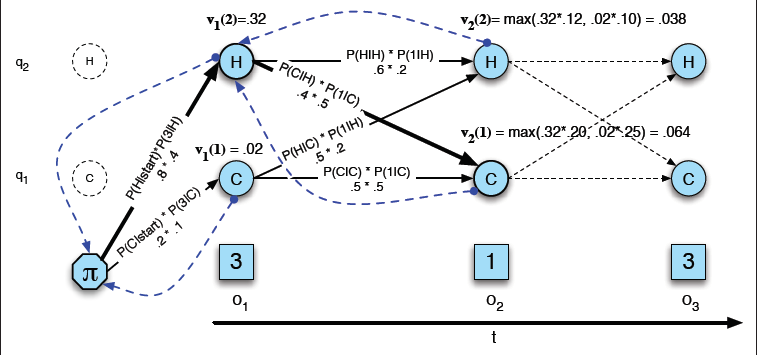
\includegraphics[scale=1]{viterbi/fig2}
\end{center}
\caption{Viterbi backtrace \label{viterbi_fig2}}
\end{figure}

Ta có định nghĩa của thuật toán Viterbi như sau:
\begin{enumerate}
\item Khởi tạo:
$${v_1}\left( j \right) = {\pi _j}{b_j}\begin{array}{*{20}{c}}
  {}&{1 \leqslant j \leqslant N} 
\end{array}$$
$$b{t_1}\left( j \right) = 0\begin{array}{*{20}{c}}
  {}&{1 \leqslant j \leqslant N} 
\end{array}$$
\item Đệ quy:
$${v_t}\left( j \right) = \mathop {\max }\limits_{i = 1}^N \left( {v{}_{t - 1}\left( i \right){a_{ij}}{b_j}\left( {{o_t}} \right)} \right)\begin{array}{*{20}{c}}
  {}&{1 \leqslant j \leqslant N,1 < t \leqslant T} 
\end{array}$$
$$b{t_t}\left( j \right) = \mathop {\max }\limits_{i = 1}^N \left( {v{}_{t - 1}\left( i \right){a_{ij}}{b_j}\left( {{o_t}} \right)} \right)\begin{array}{*{20}{c}}
  {}&{1 \leqslant j \leqslant N,1 < t \leqslant T} 
\end{array}$$
\item Kết thúc:\\
\begin{center}
Xác suất tốt nhất: $P* = \mathop {\max }\limits_{i = 1}^N \left( {{v_T}\left( i \right)} \right)$\\
Điểm bắt đầu của con đường tốt nhất: $q_T* = \mathop {\arg \max }\limits_{i = 1}^N \left( {{v_T}\left( i \right)} \right)$
\end{center}
\end{enumerate}
\textbf{Đánh giá độ phức tạp của thuật toán Viterbi:}
\begin{enumerate}
\item Độ phức tạp thời gian:
\begin{itemize}
\item Ở bước khởi tạo, ta duyệt qua lần lượt các trạng thái đánh số từ $1$ đến $N$ nên độ phức tạp thời gian ở bước này là $O \left( N \right).$
\item Ở bước đệ quy, ta dùng 2 vòng lặp lồng nhau. Vòng lặp trong có độ phức tạp  $O \left( N^2 \right),$ còn vòng lặp ngoài có độ phức tạp  $O \left( T \right).$ Như vậy, độ phức tạp của bước này là $O \left( {T \cdot N^2} \right).$
\item Ở bước kết thúc, độ phức tạp của bước này là $O \left( N \right).$ 
\end{itemize}
Như vậy, độ phức tạp thời gian của thuật toán Viterbi là $O \left( {T \cdot N^2} \right).$
\item Độ phức tạp không gian của thuật toán này là $O \left( {T \cdot N} \right).$
\end{enumerate}

\subsection{Cho một chuỗi quan sát, giả sử ta cho rằng chuỗi quan sát này được sinh ra từ một mô hình Markov ẩn với tham số chưa biết, thuật toán Baum $-$ Welch được dùng để ước lượng các tham số này. Thuật toán Baum $-$ Welch là trường hợp đặc biệt của thuật toán Kỳ vọng $-$ Tối ưu (Expectation $-$ Maximization, hay EM). Thuật toán này gồm 2 bước: bước E (Expectation, hay Kỳ vọng) và bước M (Maximization, hay Tối ưu).}
\subsubsection{Mô tả thuật toán Kỳ vọng $-$ Tối ưu tổng quát.}
Thuật toán EM là một thuật toán tuần tự (iterative algorithm), dùng để tìm kỳ vọng ban đầu cho các xác suất, sau đó sử dụng những kỳ vọng này để tìm những kỳ vọng tốt hơn, cứ tiếp tục như vậy, cải thiện giá trị xác suất học được một cách tuần tự.\\
Mô tả thuật toán Kỳ vọng $-$ Tối ưu: \supercite{g4gem}
\begin{enumerate}
\item Cho một tập hợp dữ liệu chưa hoàn chỉnh (incomplete data), xét một tập hợp các tham số khởi đầu (starting parameters).
\item Bước Kỳ vọng (bước E): sử dụng các dữ liệu đã được quan sát sẵn từ tập dataset, dự đoán giá trị các dữ liệu bị khuyết.
\item Bước Tối ưu (bước M): Dữ liệu hoàn chỉnh từ bước Kỳ vọng được sử dụng để cập nhật giá trị các tham số.
\item Lặp lại bước 2 và bước 3 cho đến khi hội tụ về giá trị tối ưu.
\end{enumerate}
\subsubsection{Mô tả và đánh giá độ phức tạp của bước E và bước M của thuật toán Baum $-$ Welch}
Trong thực tế, nhiều trường hợp ta không thể biết số lượng của bất kỳ một trạng thái ẩn nào. Thuật toán Baum $-$ Welch xử lý vấn đề này bằng cách dự đoán các số lượng này một cách tuần tự. Ta bắt đầu bằng việc dự đoán xác suất chuyển và quan sát, sau đó sử dụng các kết quả này để tìm những xác suất tốt hơn. Ta tiếp tục bằng việc tính xác suất tiến trước (forward probability) cho một quan sát, sau đó chia khối lượng xác suất (probability mass) cho tất cả con đường dẫn tới xác suất tiến trước này.\\
Trước hết, ta cần định nghĩa khái niệm \textbf{xác suất quay lại} (backward probability). Khái niệm này chỉ xác suất nhìn thấy quan sát này từ thời điểm $t + 1$ đến cuối, biết rằng ta đang ở trạng thái $i$ tại thời điểm $t$ (và một tự động hóa $\lambda$ có sẵn):
\begin{equation}
{\beta _t}\left( i \right) = P\left( {\left. {{o_{t + 1}},{o_{t + 2}}, \ldots ,{o_T}} \right|{q_t} = i,\lambda } \right)
\label{form3}
\end{equation}
Xác suất này được tính bằng quy nạp tương tự như thuật toán tiến trước.
\begin{enumerate}
\item Khởi tạo:
	$${\beta _T}\left( i \right) = 1,\begin{array}{*{20}{c}}
  {}&{1 \leqslant i \leqslant N.} 
\end{array}$$
\item Đệ quy:
$${\beta _t}\left( i \right) = \sum\limits_{j = 1}^N {{a_{ij}}{b_j}\left( {{o_{t + 1}}} \right){\beta _{t + 1}}\left( j \right),} \begin{array}{*{20}{c}}
  {}&{1 \leqslant i \leqslant N,1 \leqslant t < T} 
\end{array}.$$
\item Kết thúc:
$$P\left( {\left. O \right|\lambda } \right) = \sum\limits_{j = 1}^N {{\pi _j}{b_j}\left( {{o_1}} \right){\beta _1}\left( j \right)} .$$
\end{enumerate}

Hình \ref{bw_fig1} sau đây minh họa các bước quy nạp tính xác suất quay lui.
\begin{figure}[H]
\begin{center}
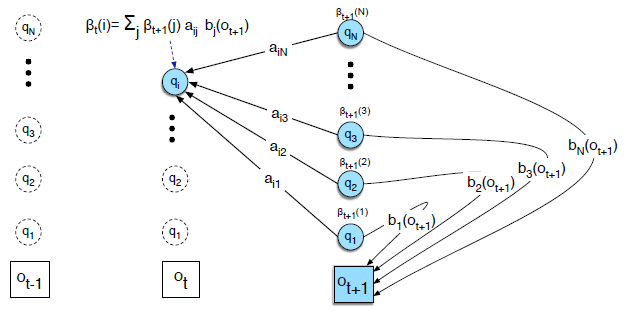
\includegraphics[scale=1]{bw/fig1}
\end{center}
\caption{Tính xác suất quay lui \label{bw_fig1}}
\end{figure}
Ta sẽ xem xét cách mà xác suất tiến trước và xác suất quay lui giúp ta tính xác suất chuyển $a_{ij}$ và xác suất quan sát $b_i \left( {o_t} \right)$ từ một chuỗi quan sát, ngay cả khi con đường thật sự trong mô hình bị ẩn.\\
\begin{equation}
\widehat {{a_{ij}}} = \frac{\text{giá trị kỳ vọng của số lượng chuyển đổi từ trạng thái } i \text{ sang trạng thái } j}{\text{giá trị kỳ vọng của số lượng chuyển đổi từ trạng thái } i}.
\label{form4}
\end{equation}
Ta định nghĩa ${\xi _t}$ là xác suất xảy ra trạng thái $i$ tại thời điểm $t$ và trạng thái $j$ tại thời điểm $t + 1,$ biết trước mô hình và chuỗi quan sát.
\begin{equation}
{\xi _t \left( {i, j} \right)} = P\left( {\left. {{q_t} = i,{q_{t + 1}} = j} \right|O,\lambda } \right).
\end{equation}
Quá trình tính giá trị này được minh họa trong hình \ref{bw_fig2}.
\begin{figure}[H]
\begin{center}
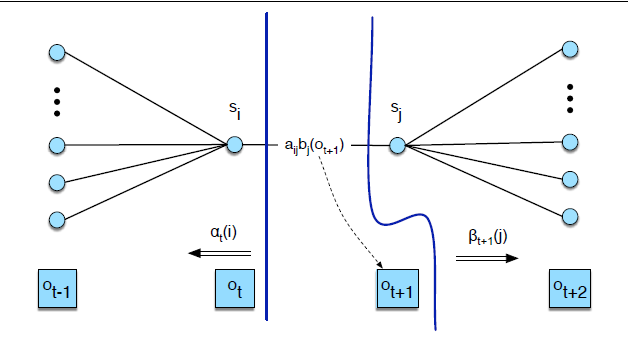
\includegraphics[scale=1]{bw/fig2}
\end{center}
\caption{Tính xác suất $\xi_t \left( {i, j} \right).$ Rabiner \copyright 1989 IEEE \label{bw_fig2}}
\end{figure}
Sau một vài bước biến đổi (\cite{hmm2021}), ta được công thức tính $\xi_t$ như sau:
\begin{equation}
{\xi _t}\left( {i,j} \right) = \frac{{{\alpha _t}\left( i \right){a_{ij}}{b_j}\left( {{o_t} + 1} \right){\beta _{t + 1}}\left( j \right)}}{{\sum\limits_{j = 1}^N {{\alpha _t}\left( j \right){\beta _t}\left( j \right)} }}.
\end{equation}
Số lượng chuyển đổi kỳ vọng từ trạng thái $i$ sang trạng thái $j$ là tổng theo $t$ của các giá trị $\xi.$ Với công thức (\ref{form4}), ta chỉ cần thêm tổng các chuyển đổi từ trạng thái $i.$ Ta có thể thu được giá trị này bằng cách tìm tất cả giá trị chuyển ra từ $i.$ Công thức cho $\widehat{a_{ij}}$ như sau:
\begin{equation}
\widehat {{a_{ij}}} = \frac{{\sum\limits_{t = 1}^{T - 1} {{\xi _t}\left( {i,j} \right)} }}{{\sum\limits_{t = 1}^{T - 1} {\sum\limits_{k = 1}^N {{\xi _t}\left( {i,k} \right)} } }}.
\label{form5}
\end{equation}
Ngoài ra, ta còn cần tìm xác suất quan sát. Đây là xác suất của một biểu tượng (symbol) $v_k$ từ bộ từ vựng quan sát (observation vocabulary) $V,$ với trạng thái $j$ biết trước: $\widehat{b_j}\left( {v_k} \right).$ Ta sẽ tính:
\begin{equation}
\widehat {{b_j}}\left( {{v_k}} \right) = \frac{\text{số lượng kỳ vọng thời điểm có trạng thái } j \text{ và biểu tượng quan sát} v_k}{\text{số lượng các thời điểm có trạng thái } j}.
\end{equation}
Ta định nghĩa $\gamma_t \left( j \right)$ là xác suất ở trạng thái $j$ tại thười điểm $t:$
\begin{equation}
{\gamma _t}\left( j \right) = P\left( {\left. {{q_t} = j} \right|O,\lambda } \right).
\end{equation}
Quá trình tính giá trị này được minh họa trong hình \ref{bw_fig3}.
\begin{figure}[H]
\begin{center}
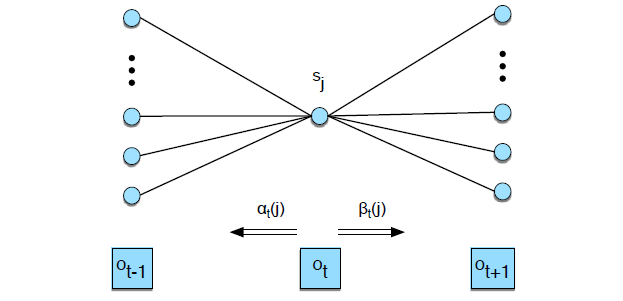
\includegraphics[scale=1]{bw/fig3}
\end{center}
\caption{Tính xác suất $\gamma_t \left( j \right).$ Rabiner \copyright 1989 IEEE \label{bw_fig3}}
\end{figure}
Sau một vài bước biến đổi (\cite{hmm2021}), ta được công thức tính $\gamma_t \left( j \right)$ như sau:
\begin{equation}
{\gamma _t}\left( j \right) = \frac{{{\alpha _t}\left( j \right){\beta _t}\left( j \right)}}{{P\left( {\left. O \right|\lambda } \right)}}.
\end{equation}
Từ đó, ta có công thức tính $\widehat {{b_j}}\left( {{v_k}} \right)$ như sau:
\begin{equation}
\widehat {{b_j}}\left( {{v_k}} \right) = \frac{{\sum\nolimits_{t = 1\begin{array}{*{20}{c}}
  {}&{s.t.{O_t} = {v_k}} 
\end{array}}^T {{\gamma _t}\left( j \right)} }}{{\sum\nolimits_{t = 1}^T {{\gamma _t}\left( j \right)} }}.
\label{form6}
\end{equation}
Giờ chúng ta có công thức (\ref{form5}) và công thức (\ref{form6}) để \textit{dự đoán lại} (re-estimate) ma trận xác suất chuyển $A$ và ma trận xác suất phụ thuộc trạng thái $B$ từ một chuỗi quan sát $O,$ giả sử ta đã có dự đoán trước đó của $A$ và $B.$\\
Các thao tác dự đoán này là lõi (core) của thuật toán Baum $-$ Welch. Thuật toán này bắt đầu từ một vài dự đoán ban đầu của các tham số mô hình Markov ẩn $\lambda = \left( {A, B} \right).$  Sau đó, ta sẽ chạy tuần tự 2 bước. Giống như các trường hợp khác của thuật toán EM, thuật toán Baum $-$ Welch có 2 bước: bước E và bước M.\\
Ở bước E, ta tính giá trị chiếm giữ trạng thái kỳ vọng (expected state occupancy count) $\gamma$ và giá trị chuyển trạng thái kỳ vọng (expected state transition count) $\xi$ từ các xác suất $A$ và $B$ trước đó.\\
Ở bước M, ta sử dụng $\gamma$ và $\xi$ để tính giá trị $A$ và $B$ mới.
\begin{breakablealgorithm}
  \caption{Thuật toán Baum $-$ Welch}
  \begin{algorithmic}[1]
    \Function{Baum-Welch}{$observation \text{ of len } T, output \text{ } vocabulary \text{ } V, hidden \text{ } state \text{ } set \text{ } Q$} 
   	\State \textbf{khởi tạo} $A$ và $B$
   	\State \textbf{duyệt} đến khi hội tụ
   	\State \Comment{Bước E}
	\State ${\gamma _t}\left( j \right) = \frac{{{\alpha _t}\left( j \right){\beta _t}\left( j \right)}}{{{\alpha _T}\left( {{q_F}} \right)}},\begin{array}{*{20}{c}}
  {}&{\forall t,j} 
\end{array}$
	\State ${\xi _t}\left( {i,j} \right) = \frac{{{\alpha _t}\left( i \right){a_{ij}}{b_j}\left( {{o_{t + 1}}} \right){\beta _{t + 1}}\left( j \right)}}{{{\alpha _T}\left( {{q_F}} \right)}},\begin{array}{*{20}{c}}
  {}&{\forall t,i,j} 
\end{array}$
     \State \Comment {Bước M}
     \State ${\widehat a_{ij}} = \frac{{\sum\limits_{t = 1}^{T - 1} {{\xi _t}\left( {i,j} \right)} }}{{\sum\limits_{t = 1}^T {\sum\limits_{k = 1}^N {{\xi _t}\left( {i,k} \right)} } }}$
     \State $\widehat {{b_j}}\left( {{v_k}} \right) = \frac{{\sum\nolimits_{t = 1\begin{array}{*{20}{c}}
  {}&{s.t.{O_t} = {v_k}} 
\end{array}}^T {{\gamma _t}\left( j \right)} }}{{\sum\nolimits_{t = 1}^T {{\gamma _t}\left( j \right)} }}$
     \State
    \Return $A, B$
    \EndFunction
  \end{algorithmic}
\end{breakablealgorithm}
\textbf{Đánh giá độ phức tạp của thuật toán Baum $-$ Welch:}
\begin{enumerate}
\item Độ phức tạp thời gian:
\begin{itemize}
\item Bước E: bước E gồm 2 phần, phần đầu có độ phức tạp $O \left( {NT} \right),$ phần sau có độ phức tạp $O \left( {N^2T} \right)$ nên độ phức tạp của bước E là $O \left( {N^2T} \right).$
\item Bước M: bước M gồm 2 phần, phần đầu có độ phức tạp $O \left( {N^2T} \right),$ phần sau có độ phức tạp $O \left( {NVT} \right)$ nên độ phức tạp của bước M là $O \left( {N^2T} \right).$
\end{itemize}
\item Độ phức tạp không gian:
\begin{itemize}
\item Bước E: $O \left( {N^2T} \right).$
\item Bước M: $O \left( {N^2} \right).$
\end{itemize}
\end{enumerate}
\newpage
%\section{Tài liệu tham khảo}
\printbibliography[title = Tài liệu tham khảo]

\end{document}